		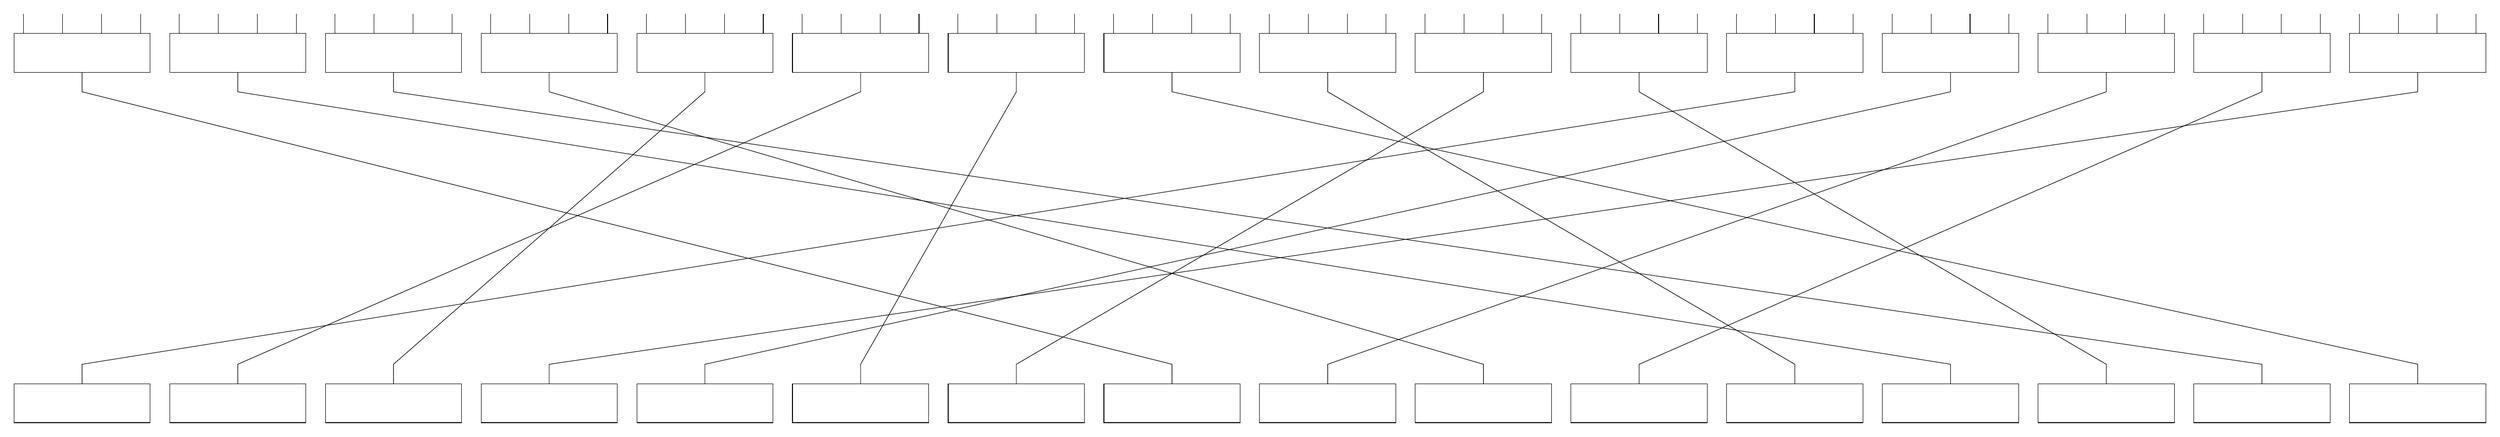
\begin{tikzpicture}
			\tikzset{
				mynode/.style={rectangle,draw=black, thick, inner sep=1em, minimum size=3em, text centered, minimum width=2cm},
				mynodep/.style={rectangle,text centered, minimum width=0.5cm, minimum height=1.1cm},
				myarrow/.style={->, >=latex', shorten >=1pt, very thick},
				mylabel/.style={text width=7em, text centered}
			}


			\foreach \x in {0, ..., 63} {
				\draw [black] (\x,20) -- (\x,19);
			}

			\def \toside {4}
			\foreach \x in {0, ..., 15} {
				\draw [black,fill=white] (-0.25+\x*\toside,19.5) -- (3.25+\x*\toside,19.5) -- (3.25+\x*\toside,18.5) -- (-0.25+\x*\toside,18.5) -- cycle;
			}

			\foreach \x in {0, ..., 15} {
				\draw [black,fill=white] (-0.25+\x*\toside,10.5) -- (3.25+\x*\toside,10.5) -- (3.25+\x*\toside,9.5) -- (-0.25+\x*\toside,9.5) -- cycle;
			}

			\foreach \i [count=\xi] in {7, 12, 14, 9, 2, 1, 5, 15, 11, 6, 13, 0, 4, 8, 10, 3} {
				\draw (\xi*\toside-\toside+1.5,18.5) -- (\xi*\toside-\toside+1.5,18) -- (\i*\toside+1.5,11) -- (\i*\toside+1.5,10.5);
			}

			% \node[mynodep] (t1) {$t_1$};
			% \node[mynodep,right=0.5cm of t1] (Op1) {$\bigoplus$};
			% \node[mynodep,right=0.5cm of Op1] (t1p) {$t_1'$};
			% \node[mynodep,right=of t1p] (A1) {$= \Delta_1$};

			% \node[mynode, below=0.5cm of t1] (f) {$f$};
			% \node[mynode, below=0.5cm of t1p] (fp) {$f$};

			% \node[mynodep,below=0.5cm of f] (t2) {$t_2$};
			% \node[mynodep,right=0.5cm of t2] (Op2) {$\bigoplus$};
			% \node[mynodep,right=0.5cm of Op2] (t2p) {$t_2'$};
			% \node[mynodep,right=of t2p] (A2) {$= \Delta_2$};

			% \draw[myarrow] (t1.south) -- (f.north);
			% \draw[myarrow] (t1p.south) -- (fp.north);
			% \draw[myarrow] (f.south) -- (t2.north);
			% \draw[myarrow] (fp.south) -- (t2p.north);
		\end{tikzpicture}
